\setRL
\clearpage
\pagenumbering{arabic} 

در این بخش تمام اطلاعات مدل‌سازی غشای لیپیدی را می‌نویسم.
\section{
بررسی مدل‌ها شبیه‌سازی غشای سلولی.
}
\subsection{
بیولوژی غشا و ساختار آن
}
\subsection{
بررسی مدل گومپر-کرول
}
گومپر
\LTRfootnote{Gompper} 
و کرول
\LTRfootnote{Kroll}
یکی از مهم‌ترین مدل‌های شبیه‌سازی غشای لپیدی رو حدود ۲۵ سال پیش ارا‌ئه دادند. می‌توان رفتار و ساختار پیچیده‌ی بسیاری از غشاها را با کشسانی لایه‌های تشکیل دهنده‌اش مدل سازی کرد مانند غشای گلبول‌های قرمز و فصل مشترک آب و روغن. همانند دو مثال گذشته اگر در غشا کشش سطحی بسیار کم باشد می‌توان رفتار ان را فقط با انرژی کشسانی خمش آن مدل سازی کرد. انرژی غشایی که خمش ذاتی ندارد را می‌توان به شکل زیر نوشت:
 




وظیفه‌ی اصلی بسته بندی $DNA$ در کروماتین به عهده‌ی هیستون\LTRfootnote{Histone} است\cite{Hammond:2017sp}. هیستون معمولا در سلول‌های دارای هسته دیده می‌شود.

\begin{figure}[h]
\begin{center}
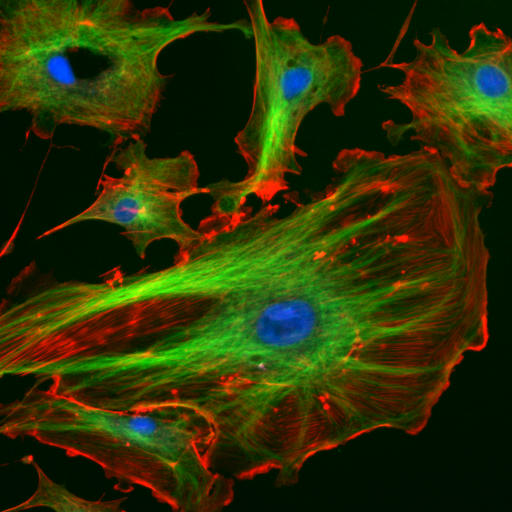
\includegraphics[width=4in]{FluorescentCells}
\caption{
تصویر سلول اندوتلیال (Endothelial) زیر میکروسکوپ نشان داده شده‌است. در این عکس  ناحیه آبی هسته سلول،‌ سبز میکروتیوبول‌ها و قرمز فیلامنت‌های اکتین را نشان می‌دهد.\cite{wiki-cell}
}
\label{fig:wiki-cyto}
\end{center}
\end{figure}

\begin{equation}
fdx=dU-TdS.\label{eq:second_thermo}
\end{equation}

\begin{equation}
\begin{aligned}
\sigma=\sigma(t_1)+\sigma(t_2) \\
\gamma=\gamma(t_1)+\gamma(t_2)
\end{aligned}
\end{equation}


\clearpage
\section{منابع}

\unsetRL
%\renewcommand{\refname}{whatever}
%\bibliography{reference} 
%\bibliographystyle{IEEEtran}
%\renewcommand\refname{مراجع}


	        
	       